% dibuix_cilindre_1.tex
\documentclass{standalone}
\usepackage{tikz}
\usetikzlibrary{arrows.meta, decorations.markings}

\begin{document}

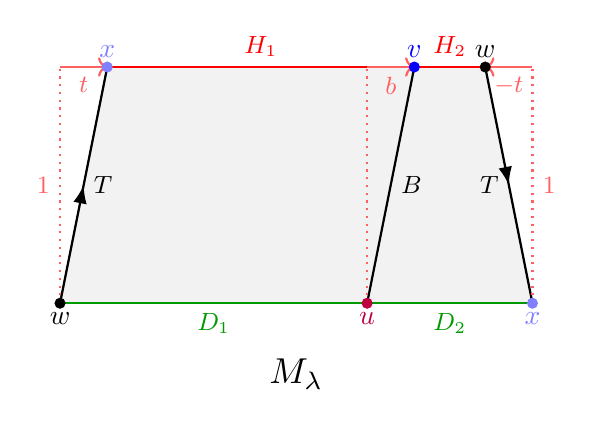
\begin{tikzpicture}[
    identified_edge/.style={
        decoration={
            markings,
            mark=at position 0.5 with {\arrow{Latex}}
        },
        postaction={decorate}
    },
    edge_label/.style={midway, auto, font=\small}
]

\def\squaresize{3}
\fill[gray!10] (0,0) -- (0.2 * \squaresize,\squaresize) -- (1.8 * \squaresize,\squaresize) -- (2 * \squaresize,0) -- cycle;
\draw[identified_edge, thick] (0,0) -- node[edge_label, right] {$T$} (0.2 * \squaresize,\squaresize);
\draw[identified_edge, thick] (1.8 * \squaresize,\squaresize) -- node[edge_label, left] {$T$} (2 * \squaresize,0);

\draw[thick] (1.3 * \squaresize,0) -- node[edge_label, right] {$B$} (1.5 * \squaresize,\squaresize);

\draw[red, thick] (0.2 * \squaresize,\squaresize) -- node[edge_label, above] {$H_1$} (1.5 * \squaresize,\squaresize);
\draw[red, thick] (1.5 * \squaresize,\squaresize) -- node[edge_label, above] {$H_2$} (1.8 * \squaresize,\squaresize);
\draw[green!60!black, thick] (0,0)       -- node[edge_label, below] {$D_1$} (1.3 * \squaresize,0);
\draw[green!60!black, thick] (1.3 * \squaresize,0)       -- node[edge_label, below] {$D_2$} (2 * \squaresize,0);
\draw[pink!50!red, dotted, thick] (0,0)       -- node[edge_label, left]  {1} (0,\squaresize);
\draw[pink!50!red, dotted, thick] (1.3 * \squaresize,0)       -- node[edge_label, left]  {} (1.3 * \squaresize,\squaresize);
\draw[pink!50!red, dotted, thick] (2 * \squaresize,0) -- node[edge_label, right] {1} (2 * \squaresize,\squaresize);

\draw[pink!50!red, ->, thick] (0,\squaresize) -- node[edge_label, below] {$t$} (0.2 * \squaresize,\squaresize);
\draw[pink!50!red, ->, thick] (2 * \squaresize,\squaresize) -- node[edge_label, below] {$-t$} (1.8 * \squaresize,\squaresize);
\draw[pink!50!red, ->, thick] (1.3 * \squaresize,\squaresize) -- node[edge_label, below] {$b$} (1.5 * \squaresize,\squaresize);

\node[scale=1.3] at (1 * \squaresize,-0.3*\squaresize) {$M_\lambda$};
\fill[purple] (1.3 * \squaresize,0) circle (2pt) node[below] {$u$};
\fill[black] (0,0) circle (2pt) node[below] {$w$};
\fill[blue!50] (2 * \squaresize,0) circle (2pt) node[below] {$x$};
\fill[blue!50] (0.2 * \squaresize,\squaresize) circle (2pt) node[above] {$x$};
\fill[blue] (1.5 * \squaresize,\squaresize) circle (2pt) node[above] {$v$};
\fill[black] (1.8 * \squaresize,\squaresize) circle (2pt) node[above] {$w$};
% \fill[blue] (\circle_size,0) circle (2pt);

\end{tikzpicture}

\end{document}